
\section{Conclusions and Contributions}\label{conc:sec:research-conclusions}

Our primary job as evolutionary archaeologists is to document the course of cultural evolution, by mapping heritable continuity from archaeological remains.  That job employs many tools, both new and old, from phylogenetic and cladistic methods still under development today, to seriation and classification methods now more than a century old.  Cultural transmission, broadly speaking, is the central organizing concept which explains why there is heritable continuity to be found in the spatial and temporal variation in artifact form.  It is natural for us to employ mathematical models of diffusion and transmission to attempt to understand cultural transmission better.  

In Chapter \ref{chap:introduction} I described three different research programs within archaeology on cultural transmission, distinguished by the spatiotemporal scale of their focus.  The first, a ``microevolutionary'' program, stemmed from two different sets of questions.  The first sought to determine whether particular assemblages or groups of assemblages showed evidence of selection, by testing the null hypothesis that class frequencies met some criterion derived from neutral models borrowed from population genetics.  The second sought to go beyond simply testing for neutrality and attempt to fit psychological models of biased social learning, derived from Boyd and Richerson's seminal work, to assemblage data.  Although neither question is necessarily synchronic by nature, the models and statistical approaches employed have tended to be.  In Chapters \ref{chap:timeaveraging-paper} and \ref{chap:ctmixtures-paper} I studied the question of whether the microevolutionary program could be made empirically sufficient and thus useful for answering detailed questions about the archaeological record.  In Section \ref{conc:sec:conc-microevolutionary} I review my conclusions and highlight contributions from this work which have not appeared elsewhere in the literature.

Much of that work was methodological and critical in nature.  My work with Robert Dunnell and others from the University of Washington's sphere of influence within evolutionary archaeology led me to believe that the microevolutionary program all too easy led to synchronic, reconstructionist analyses that did not take advantage of our unique strength:  time depth.  The mesoscopic and macroevolutionary programs described in Chapter \ref{chap:introduction} are both broadly diachronic in focus, and differ mainly in spatiotemporal scale and the methods uses.  My main contribution in this dissertation has been to further develop elements of a true ``mesoscale'' approach to mapping heritable continuity, distinct from the strong focus of macroevolutionary analysis on the use of phylogenetic techniques.  In Sections \ref{conc:sec:conc-seriation} and \ref{conc:sec:conc-structured} I review my conclusions and highlight unique contributions from this research program.  Further, in Section \ref{conc:sec:final-thoughts}, I return to the relationship between the ``mesoscale'' and macroevolutionary programs, and discuss the key role of classification in determining where a particular research problem lies in the continuum between meso and macro. 

The ``mesoscale'' approach I have sought (in collaboration with Carl Lipo) to develop employs time-honored archaeological methods, updated for a new century and the computing power we now have available, but in conceptual terms is still in its infancy.  We are still exploring what the right structure is for transmission models at this scale, given different kinds of archaeological situations.  There is considerable scope to elaborate not only the methods described in this dissertation, but develop new observable units and models.  In Section \ref{conc:sec:future-research}, I outline what I believe to be fruitful next steps to advance elements of this research program.

\subsection{Microevolutionary Cultural Transmission Models in Archaeology}\label{conc:sec:conc-microevolutionary}

Despite the fact that archaeology understands itself as studying cultural \emph{change} through the archaeological record, we routinely (and often inadvertently) find ourselves describing the past in ways that are synchronic and essentialized.  Even though Nels Nelson \citeyearpar{Nelson1916} clearly articulated a diachronic view of stylistic change in his work at San Crist\'obal, later pratice in ``culture history'' framed our knowledge of the past as a series of synchronic snapshots.  \emph{Change} through time became represented as mere \emph{difference} between period or phases, and theoretical effort shifted to the reconstruction of the ``Indian behind the artifact'' \citep[79]{braidwood1959archeology}.  

The pull of synchronic description and the reconstructionist enterprise of describing the state of a population at a moment in time is no accident---it is built into the way we perceive the world and organize our knowledge.   \citet{Dunnell1982} described the cognitive biases that lead to this tendency as our ``common sense'', which constructs views of the world consistent with the short time scales over which we need to perceive the world and adapt.  Social and cognitive psychologists have since begun to document the proximate causation for essentialized cognition in early development \citeeg{Rhodes13526,rhodes2017development,gelman2004psychological}.  

Indeed, our tendency to think about the world in synchronic and essentialized terms is so strong that Mayr, Lewontin, and others have argued that the primary revolution Darwin kicked off was not about evolution itself, or even the theory of natural selection, but through the introduction of ``population thinking'' as an alternative to the typological, essentialist thinking about species and the nature world that characterized pre-Darwinian biology \citep{Dunnell1982,lewontin1974darwin,Mayr1959typological}.  The ``materialist revolution,'' as Lewontin termed it, treated \emph{variation} as causal, rather than noise, and required one to think about change in fully diachronic terms.  Evolutionary archaeology began with Dunnell's articulation of exactly this point \citep{Dunnell1978,Dunnell1980,Dunnell1982,Dunnell1989}.  

Despite this, the application of cultural transmission models within evolutionary archaeological very quickly took on a synchronic, ``reconstructionist'' flavor.  By adopting equilibrium models from classical population genetics, whether the Wright-Fisher model of drift or the social psychological models from Boyd and Richerson's justifiably influential work \citeyearpar{BR1985}, the very structure of the models themselves gave predictions for the stationary, unchanging state of a population.  Fitting such models to observational data requires treating our data ``as if'' they were a synchronic sample of a population at a moment in time, so that the observed frequency distribution can be compared to the theoretical one.  Nearly all of the microevolutionary program for cultural  transmission modeling in archaeology has proceeded in this way, until very recently \citep{Kandler2013}. 

Chapter \ref{chap:intro} describes in more detail how, as researchers began to see conflicting results when reanalyzing the same canonical data sets over and over in their methodological papers, it became apparent that efforts to fit cultural transmission models to data led to ambiguous conclusions.  This realization led to serious discussion about equifinality between transmission models \citep{barrett2019equifinality,kandler2019analysing,premo2010equifinality}.  The first set of questions that comprise this dissertation address this question:  how severe are  the equifinality problems faced by the microevolutionary approach?  Is it possible to distinguish between transmission models using coarse-grained data on frequencies of cultural traits in a population?

Archaeological data are ``coarse grained'' in two ways, both relevant to the microevolutionary program.  The first is that archaeological observations are always diachronic in nature and inherently represent counts and frequencies that refer to depositional events over a duration.  Sometimes the duration might be short, as in the archaeological record of recent historical periods, or a single assemblage may represent deposition across millennia.  Second, as archaeologists we nearly always operate with assemblages which represent whole populations or subpopulations, except in specific depositional and many historical contexts.  This means that heterogeneity within populations may not be distinguishable given assemblage-level data.  Furthermore, this means that realistic models of heterogeneous social learning may not be identifiable and empirically sufficient with population level data alone.  Chapters \ref{chap:timeaveraging-paper} and \ref{chap:ctmixtures-paper} addressed each of these types of ``coarse graining'' on our ability to fit cultural transmission models.  I summarize their conclusions in turn.

\subsubsection{The Centrality of Time Averaging To Evolutionary Modeling}\label{conc:sec:conc-timeaveraging}

Chapter \ref{chap:timeaveraging-paper} examined the effect of time averaged observations on the observable statistics we use to measure goodness of fit between archaeological frequency distributions, and the theoretical models we employ as hypotheses.  Since most of our hypothesis tests or goodness of fit testing is related to the shape of frequency distributions, the effect of aggregation on diversity measures is critical to understand.  My results indicate that richness is inflated in samples with longer duration compared to synchronic observations.  This is the underlying reason why culture historians noted that assemblages used in seriation should be of equal duration.  But this fact takes on critical importance with most of our cultural transmission models, since the number of expected traits (or alleles, given their origin in population genetics) is the ``sufficient statistic'' at a given population size and mutation rate.  The ``evenness'' of frequencies is flattened with greater assemblage duration; this causes problems with neutrality tests that seek to employ the shape of the frequency distribution, including Ewens and Watterson's tests and Slatkin's ``exact'' tests for neutrality.  As a result, such tests display increased Type I error rates.  

The most important contribution of Chapter \ref{chap:timeaveraging-paper} is the linkage between how long cultural traits persist in the record, and the timescale over which time averaging effects appear.  Assemblages whose duration is longer than the mean lifetime of the classes which analytically represent cultural variation will display increased richness, flattened diversity, and increased Type I error in ``neutrality tests.''  Assemblages whose duration is equal to the mean trait lifetime, or shorter, are not affected by time averaging in these ways measured here.  This is an important result because archaeologists can, at the time of data collection and subsequent artifact analysis, exert some control over the effects that time averaging might have on our analyses.  Relative comparisons between assemblages are possible, if durations are relatively comparable.  Sometimes it is possible to control the degree to which we aggregate artifacts into ``assemblages'' for analysis both during fieldwork, and afterwards in an analytical manner.  Assemblage duration is not fully controllable in this manner, of course, but to date this has not be a variable which has entered into the application of cultural transmission analysis.  

In like manner, we have partial control over the relative lifetimes of the artifact classes we use to measure cultural variation.  We must always remember that the classes and types whose frequencies we are comparing to transmission models are analytical constructions, rather than being inherent in the rocks and sherds we handle themselves \citep{Dunnell1971}.  Because we form the classes we then use for counting abundance and forming frequency distributions, we can vary classification ``level'' (\emph{sensu} \citealt{Dunnell1971}) and vary the amount of time over which we observe a class.  Varying the number of dimensions of variation in our classification will affect the measured ``lifetime'' of the classes themselves.  Individual attributes (or modes) belonging to a single dimension of variation (e.g., straight rims on ceramic bowls) may persist in the archaeological record for long periods of time (and, indeed, by themselves may occur in unrelated contexts, thus being non-homologous).  But when we combine dimensions of variation, say by constructing a ceramic classification by intersecting rim form with surface treatment with rim decoration, each combination of these dimensions tends to have a restricted spatio-temporal distribution.  Since we can affect our classifications and the level of detail they differentiate, we have some ability to tune our observations of cultural trait frequencies in response to the level of temporal aggregation present in the archaeological deposits we seek to study.  

This does not mean that careful tuning of classification level, and reduction of assemblage duration is sufficient to render synchronic, microevolutionary models empirically sufficient.  Even short duration assemblages are still a diachronic source of data, that demand diachronic, historical explanations.  The effects of time averaging are worth studying not because we can ``correct'' for them, but because aggregation effects tell us something about the time scales our diachronic hypotheses must be frame at, in order for our data not to ``underdetermine'' alternative models \citep{perreault2019quality}.  The study of time averaging effects is integral if an evolutionary archaeology is to develop testable explanations for the archaeological record, as it is critical for paleobiology to develop testable explanations of the fossil record \citep{kowalewski1996time}.


\subsubsection{Coarse Grained Data Cannot Distinguish Realistic Microevolutionary Models}\label{conc:sec:conc-ctmixtures}

Chapter \ref{chap:ctmixtures-paper} examined the second problem that the microevolutionary approach faces given only coarse grained data sources.  Data on artifact class frequencies nearly always reflect prevalence in some population aggregate, with only limited information about individual variation (except in historical archaeology and certain other specialized depositional circumstances). 
Since real human (and animal) populations are a mixture of individuals with different social learning strategies, we need to understand the degree to which heterogeneous populations are reflected in population-level aggregated data in ways that can be statistically identified.  Or whether population-level data ``average over'' individual variation in ways that cause population-level patterns to converge too strongly to differentiate between models.
Using simulation and machine learning classifiers, I examined whether it was possible to distinguish \emph{different} mixtures of social learning strategies with only population-level summary data, in the form of relative frequencies of artifact classes.

The results were not encouraging, if population level data are also subject to sample size effects and any temporal aggregation.  It proved possible in some cases to distinguish between mixtures of strategies and a population of the same size practicing unbiased copying, when the frequencies used were a complete census of the population, and when no aggregation was present.  With partial samples of the population, equifinality between models (even under the ideal circumstances of a simulation experiment) increased.  Similarly, when time averaging of observations is a factor, equifinality between model comparisons was strong, and with both factors, we are simply unable to distinguish between theoretical models with population-level data on trait frequencies.  This does not bode well for identification of microevolutionary models of transmission in most archaeological situations.  

\subsubsection{A Systematic Method for Measuring Equifinality and Underdetermination}\label{conc:sec:equifinality-underdetermination}

In addition to examining the limits of empirical sufficiency given population level data, Chapter \ref{chap:ctmixtures-paper} describes an explicit method for detecting equifinality among theoretical models.  In addition, the method simultaneously addresses  ways in which the spatiotemporal resolution, duration, or data collection treatments may affect empirical sufficiency.  I use the idea that distinguishable hypotheses (models) will generate predictive data distributions which can be distinguished by the \emph{Bayes classifier} for the model set; sets of models which are equifinal given a set of variables and data collection treatments will not be separable.

The Bayes classifier is typically impossible to directly calculate, but it can be well approximated by using machine learning classifiers with sufficiently high model capacity \citep{Hastie2009}.  In this study, I examined classifier performance in distinguishing pairs of transmission models, with samples from the same predictive data but with differing sample sizes and amounts of temporal aggregation.  This combination of methods allows us to examine two questions simultaneously \begin{dissparalist}
\item are a set of models or hypotheses distinguishable \emph{even in theory}, given a set of observable variables
\item how do data collection treatments, or the empirical scale of our data in terms of resolution or duration, affect model identification
\end{dissparalist}?  This method is more general than cultural transmission modeling, and in fact should be a standard question we ask about theoretical models and our data at the outset of a research project.  As \citet{perreault2019quality} notes in his excellent recent book, far too many models in archaeology are empirically insufficient because they are underdetermined by any data we can feasibly collect.  


\subsubsection{Final Thoughts on the Microevolutionary Program}\label{conc:sec:final-micro}

I started this dissertation work understanding that much of the cultural transmission modeling happening in archaeology was aimed at synchronic, reconstructionist goals; for example, attempting to determine what cognitive biases a past population might have displayed.  It should be clear that there is no good answer to that question even in theory.  Are modern communities ``conformist''?  Novelty seeking?  The answer has to be ``no'':  individuals are, and vary in that tendency, and this means the frequency and prevalence of different social learning behaviors varies both historically, and situationally.  I began this work with the goal of trying to examine larger scale ways of modeling cultural transmission, but I did wonder whether models like Boyd and Richerson's could be ``scaled up'' to gather diachronic, longer-term and larger-scale predictions (much as \citealt{Kandler2013} proposed).  

This kind of rescaling approach has been incredibly successful in other disciplines, such as statistical physics and physical chemistry.  In order to rescale (or ``renormalizing'', to use the term most often employed by physicists) our cultural transmission models, we would progressively observe them at larger scales, ``averaging'' over variation at lower scales to determine behavior at larger scales.  The research in Chapter \ref{chap:ctmixtures-paper} began with precisely this approach:  I wanted to see if an explicit renormalization approach, of the type pioneered by Leo Kadanoff \citeyearpar{Kadanoff2000}, would show that mixtures of social learning modes ``average out'' to appear unbiased.  The basic concept for this kind of renormalization is pictured schematically in Figure \ref{conc:fig:renormalizing-ct}.  To the extent that individuals ``balance'' each other's biases and social learning modes, the net effect when we ``zoom out'' may look unbiased.

\begin{figure}[ht!]
  \centering
  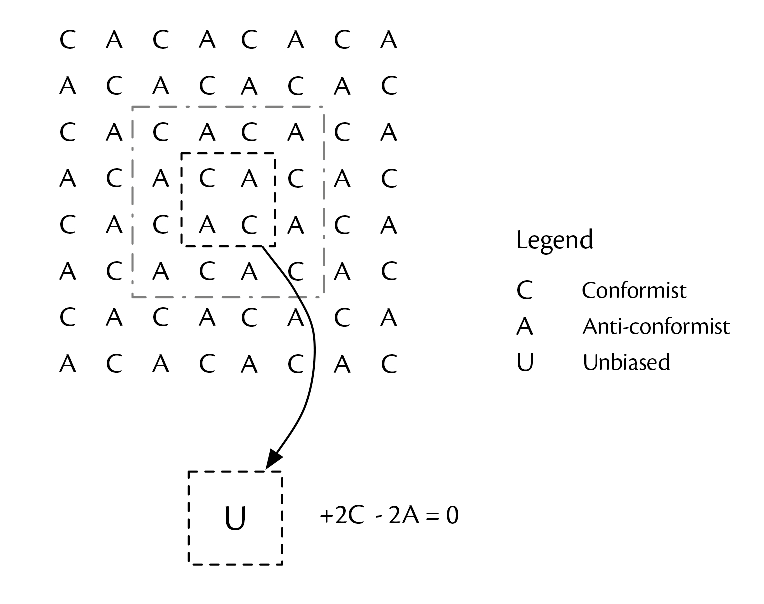
\includegraphics[scale=0.5]{graphics/conclusion/renormalizing-ct-modes.pdf}
  \caption{Example of ``block renormalization'' of a mixture of cultural transmission modes.  Under the assumption that the conformist and anti-conformist biases are either equal and opposite, or drawn from random prior distributions, as one averages over more and more individuals, the population level effect begins to look more unbiased.  This concept was the original impetus for the modeling approach taken in Chapter \ref{chap:ctmixtures-paper}.}
  \label{conc:fig:renormalizing-ct}
\end{figure}

There is certainly an inability to distinguish between mixtures of social learning modes, as documented in Chapter \ref{chap:ctmixtures-paper}, but I came to believe that an explicit renormalization approach to moving us from microevolutionary models to their mesoscopic consequences was not a fruitful one.  The ability to renormalize a theory at a lower level and use it to predict consequences at larger scales turns out to depend upon two main properties, which are quite general.  

First, ``coarse graining'' a theoretical model requires \emph{scale separation}, where some aspects of the detailed fine grained behavior of the system can be ignored at the higher level, because the effects become small enough to ignore \citep{hillerbrand2015explanation}.  A classical example is using the ``fine grained'' theory of classical mechanics to predict the behavior of planets in our solar system (the coarse grained problem). We know that the ``two body'' problem is solvable, because the interaction between two objects still produces integrals with closed-form solutions.  But even the ``three body problem'' (say, the Sun, Earth, and Moon) is not solvable.  The degrees of freedom produce non-linear interactions and the system is no longer analytically integrable.  Why then, can we still produce numerical answers with stunning accuracy?  The contributions of some forces become exponentially small, given their size and distance, and thus can be ignored.  Scale separation denotes the situation where some small scale effects become orders of magnitude smaller than the ``main'' effects in our models, and thus can be omitted.  It is not clear if this kind of scale separation is relevant to projecting the effects of individual variation in social learning and small scale population structure to regional scales and time scales of decades or centuries.  It is also not clear that it doesn't under some circumstances, so this remains an open question.

Second, usually in physical theory, the fine grained theory is ``simpler'' than the macro or mesoscale phenomena.  Classical mechanics is time reversible and follows a few simple principles; it is the mesoscale phenomena like superconductivity, magnetism, and phases of matter that display complexity, phase transitions, and ``critical points'' where their behavior flips.  The whole discipline of statistical physics aims, in fact, to understand universal principles for how combinations of simple rules give rise to complex and path-dependent behavior at large scales.  As seductive as it is (at least to me!) to think that we could apply this kind of modeling paradigm in the social sciences, it seems increasingly clear to me that we are facing a different kind of situation.  The individual scale is not simple---it is rich and variable, as much of anthropology, psychology, and other social sciences can attest.  The situation we face is less like orbital mechanics and more like the study of turbulence in fluid dynamics, where small details lead to structure and pattern at all scales.  And there is no good solution at the microscale for problems like turbulence.  We study them empirically, at the scales we need to, for the data we are attempting explain.  The mathematical problem of studying turbulence directly at the ``individual'' or micro scale remains out of reach---one of the Millennium Prize challenges, if it can be solved at all.

Thus, I have come to believe that we are in a situation where instead of employing individual-level models as explanations in themselves, our models need to directly model variation and history at mesoscopic and macroscopic scales.  
The strength of archaeology as an evolutionary discipline is time depth:  we study a record of how human behavior differs over space and has changed over time.  This requires us to construct models that are hypotheses about the evolutionary history of cultural variants in a region and over a period of time.  Our evolutionary models should be hypotheses about the trajectories that different models of cultural transmission and social learning take, over time scales which match the time scales at which we can realistically observe the process.  


\subsection{Mapping Evolutionary History at the ``Mesoscale'' with Seriation Graphs}\label{conc:sec:conc-seriation}

As we move away from microevolutionary analysis and towards historical, diachronic models at the ``mesoscale,'' the modeling framework necessarily changes.  Our hypotheses are no longer synchronic, equilibrium models but instead become historical narratives which describe why changes we see in artifact class frequencies occurred in the way they did.  \citet{OHara1988}'s distinction between ``chronicle'' and ``history'' provides the perfect framework for modeling this kind of evolutionary history.  Chronicles are ``the facts,'' while histories are explanations.  Histories provide causal narratives that purport to explain the chronicle of empirical observations. 

In Chapters \ref{chap:seriationcombinatorics-paper}, \ref{chap:multipleseriation-paper}, and \ref{chap:computational-metapopulation}, I explored how to \begin{dissparalist}
\item formalize a hypothesis about the regional history of community interaction and cultural transmission in the form of an `` temporal network'' model
\item construct seriation graphs which summarize the spatial and temporal history of how cultural traits varied 
\item develop methods for assessing the fit between a temporal network model and an empirical seriation graph, using summary statistics about seriation graph topology.
\end{dissparalist}  In this structure, a set of interval temporal network models are the candidate ``histories'', and function as hypotheses.  Seriation graphs function as one kind of evolutionary chronicle; in this case, it is a chronicle about the spatial and temporal change that we see in the frequency of different cultural traits.  Statistical properties of seriation graphs become the statistics we use in machine learning models to make judgments about equifinality, and to attempt to perform empirical fits  to data. 

In order for seriation graphs to function well as chronicles, they need to have rich enough state spaces that different causal histories will cause meaningful differences in the structure of the seriation solutions.  This is an important reason that Lipo and I moved to a graph representation from our former work building multiple independent seriations out of empirical datasets \citep{Lipo2015}.  But richness of structure means that seriations must incorporate many assemblages, not just a few.  Small seriation solutions will nearly always underdetermine any set of candidate hypotheses, because the models will often be equifinal across very small samples.  Thus, in Chapter \ref{chap:multipleseriation-paper}, I worked with Carl Lipo on developing more efficient criteria for seriating large sets of assemblages.  Our results with distance-minimization as the ordering criterion builds on earlier work by Kadane and Shepherdson, and in combination with our graph construction heuristics, yields the ability to easily analyze dozens of assemblages at a time and construction seriation graphs.  

Chapter \ref{chap:computational-metapopulation} represents an initial attempt to put the pieces described above together, and determine whether it is possible, in theory, to discern hypotheses about regional transmission history, using seriation graphs as the empirical unit of observation.  The results are positive and suggestive that further research would help outline the limits of the approach, and possibly improve discriminatory power between different classes of historical models.  I return to the next steps for this research program in Sections \ref{conc:sec:future-temporal-networks} and \ref{conc:sec:future-seriation-structure}.   

\subsection{Methods for Including Structured Information in Cultural Transmission Models}\label{conc:sec:conc-structured}

In addition to constructing better spatiotemporal models of cultural transmission at archaeological scales, we also need ``thicker'' descriptions (sensu \citealt{Geertz1973,gilbert1949concept}) of cultural variation and how social learning processes interact and coevolve with the \emph{content} of cultural variation.  Following ideas from \citet{mesoudi2008learning}, in Chapter \ref{chap:semanticaxelrod-paper} I considered how to build a model encapsulating the \emph{dependency structure} between traits in the form of a graph.  Simulated transmission dynamics were then subject to that dependency structure as well as social learning rules.  Two types of social learning rule were then compared in a modified Axelrod model:  individual innovation, as compared to direct instruction.  The results show that, as one might expect, formal instruction or tutoring results in deeper, more complete cultural repertoires, in comparison to pure imitation and individual trial-and-error learning.  This research originally appeared in a volume on the ``learning hypothesis'' for behavioral modernity among Upper Paleolithic hominids, and the results described here lend support to the idea that ``behavioral modernity''---the explosion of complexity and variety seen in late Paleolithic artifact inventories---may be the result of the coevolution of new forms of social learning with cumulative technological development, rather than being a consequence of biological change or demographics.

At a methodological level, this work contributes new ways of modeling cultural transmission such that we can create credible hypotheses for how social learning rules and content can evolve together.  This is necessary if we are going to move beyond formal, very abstract models for cultural transmission, and actually explain the evolutionary history of a technology.  The effort to construct thicker models has been championed by \citet{tostevin2019content} in archaeology, following the critically important work of William Wimsatt and colleagues \citep{wimsatt2007reproducing,wimsatt2019articulating}.  I discuss some possible future research directions in Section \ref{conc:sec:future-design-space}.

\section{Next Steps and Future Research}\label{conc:sec:future-research}

The major goal of my dissertation research is to examine whether we can improve the empirical sufficiency of cultural transmission research in archaeology by \begin{dissparalist}
\item understanding the sources of equifinality between models, and building methods to detect it;
\item modeling cultural transmission at spatial and temporal scales appropriate to the coarse grained nature of archaeological data;
\item selecting empirical observable units (such as seriation graphs) which display enough variation between models, that our hypotheses are not underdetermined.
\end{dissparalist}  The conclusions just described show, I believe, some success in achieving all three goals.  Nevertheless, some of the approaches I employed, such as the use of temporal networks and seriation graphs in Chapter \ref{chap:computational-metapopulation} remain in their infancy, with many questions still to answer and refinements possible.  In this section, I describe next steps for several of the methods and approaches used in previous chapters. 

\subsection{Further Development of Temporal Network Models as Evolutionary Hypotheses}\label{conc:sec:future-temporal-networks}

In Chapter \ref{chap:computational-metapopulation}, I examined the idea that we could represent a diachronic hypothesis about the history of cultural transmission in a region in the form of a so-called ``temporal'' or ``time-varying'' network.   
I proposed that interval temporal networks were a good tool for representing long term change in cultural transmission patterns between sedentary, nucleated communities.  The temporal network model functions as a formalization of a standard ``metapopulation'' modeling framework, in which discernible subpopulations can be identified and sampled, and have sufficient persistence that one could (in theory) measure migration rates between the subpopulations.  Not all of the empirical situations we wish to study as archaeologists fit into a metapopulation modeling strategy, however, and thus interval temporal networks will not be a good tool for representing evolutionary hypotheses in all situations.  Interval networks would not be a good structural model for transmission in highly mobile populations or dispersed hunter gatherer communities, for example.  Given how difficult it is to describe residential and community patterning in the deep Paleolithic record, we would need different empirical models for such situations, which perhaps look more like continuous fields with gradients rather than graphs with nodes and edges. 

Within the class of problems for which interval temporal networks are appropriate, there are several avenues to follow and improve upon the results reported here.  These include:

\begin{itemize}
    \item Understanding how to characterize equivalence classes of temporal network structures, in the same way that we can order or classify static graphs;
    \item Describe equivalence classes of network structures that have similar behavior under transmission or diffusion processes.
\end{itemize}

The first element involves understanding good ways to characterize meaningful differences in interval graphs.  In Chapter \ref{chap:computational-metapopulation} I did not directly analyze the temporal network models themselves, instead looking for the \emph{effect} their structure may have on transmission via seriations.  This approach, derived from my earlier work on ways to characterize equifinality (see Chapter \ref{chap:ctmixtures-paper}), is useful but highly indirect and computationally expensive.  We can complement the approach I took here with a direct study of the interval temporal networks that form our transmission scenarios.  

For static graphs, there are many results in graph theory that help characterize equivalence classes of graphs.  In particular, functions of the Laplacian spectrum define classes of structures, as do the eigenvalues of the adjacency matrix.  The ``energy'' of a graph (i.e., the sum of the eigenvalues of the adjacency matrix) appears to be strongly related to how the graph can be decomposed into subgraphs with differing structure (e.g., cycles, cliques, trees) \citep{estrada2017meaning,gutman2006laplacian}.  We also know, for example, We know that trees which have 4 or 5 distinct eigenvalues (at a given diameter) are completely characterized by their normalized Laplacian spectrum \citep{braga2015trees}.  That is, each distinct set of eigenvalues forms a distinct and distinguishable set of tree structures.  The ability to understand structural equivalence classes is important for understanding when we should see differences in the \emph{behavior} of a cultural transmission process across a set of network structures, since a large body of research has shown how graph topology affects diffusion-like processes on static graphs (see reviews in  \citealt{Castellano2006,Durrett2007,grimmett2018probability,szabo2007evolutionary}).

For time varying or temporal graphs, we are beginning to understand their structural properties \citep{nicosia2013graph,nicosia2012components}, especially given strong interest by computer scientists in using temporal contact networks to study consensus algorithms, distributed systems design, and mesh network design.  Similarly, given the importance of time varying contact networks in epidemiology, we are beginning to understand the behavior of diffusion processes across contact networks \citep{liu2013contagion,pare2017epidemic,liu2014social,uribe2019non,santoro2011time}.  Most of this work has focused on ``contact'' networks where edges represent short-duration events, so there is a need to examine the degree to which the behavior of diffusion processes on interval networks may differ from contact networks.  

Finally, given a general understanding of how diffusion processes (including epidemics, cultural transmission, population genetics) operate on interval networks, we can return to the general approach taken in Chapter \ref{chap:computational-metapopulation} and examine more systematically which transmission scenarios we can distinguish.  To answer archaeological questions about ``complex societies,'' for example, we would like to be able to formulate transmission scenarios where ``hierarchy'' exists.  We also need to be able to model the transition from flatter ``nearest neighbor'' and ``small world'' patterns of connectivity to hierarchical patterns of interaction, in order to examine hypotheses about the origins of hierarchical forms of social organization, and its potential breakdown.

\subsection{Statistical Properties of Seriation Graph Solutions and Transmission Scenarios}\label{conc:sec:future-seriation-structure}

In order to perform statistical analysis on seriation solutions, including using classifier models to under equifinality, or clustering algorithms to understand similarities in structure, we need to extract summary statistics from seriation graphs.  In Chapter \ref{chap:computational-metapopulation} I focused on the ``Laplacian spectrum'':  the set of eigenvalues and their multiplicities for the Laplacian matrix of a graph.\footnote{Concurrent with my own work, \citet{lewitus2016characterizing} employed Laplacian spectra to classify phylogenetic trees.}  The Laplacian matrix for a general graph incorporates information about the pattern of edge connections through the adjacency matrix, and the density of connectivity (or ``branchiness'', for trees) through the degree matrix.  I employed the eigenvalues of the Laplacian as a set of independent or predictor variables that I used to train a classifier model, measuring the ability to cleanly separate different graph structures and ``predict'' the true data generating model underlying the seriation graph.  

Although this approach was successful, it is not clear how many classes of transmission scenarios can be distinguished.  To understand how generic the approach might be, and what additional developments might improve it, I propose two research directions to further develop the method:

\begin{itemize}
    \item We need to characterize how much variation in Laplacian spectra exists across seriation graphs with a given number of assemblages;
    \item We can explore richer representations for seriation relationships which will provide bigger state spaces for discriminating between hypotheses.
\end{itemize}

One thing that the approach taken in Chapter \ref{chap:computational-metapopulation} did not clarify is the degree to which seriation graphs might not vary enough in their Laplacian spectra to distinguish between data generating processes.  How large is the ``state space'' formed by possible eigenvalue spectra for all trees on N vertices?  It may turn out that there is enough variation to differentiate transmission scenarios which are extremely different in their structure:  for example, nearly regular graphs of the ``nearest neighbor'' type, and a lineage splitting model which contains separate components.  What is unclear is whether seriation graphs are still ``too similar'' in structure such that they underdetermine more subtle comparisons between transmission scenarios, such as small world connections versus hierarchical social interaction.  A first step is to characterize how much the Laplacian spectra of trees with $N$ vertices can vary.  For example, although the number of uniquely labeled trees on, say, 20 assemblages is very large (Cayley's theorem yields $2.62 \times 10^{23}$ distinct solutions), the number of distinguishable spectra may be much smaller given that trees have relatively limited variation in edge connectivity patterns.  This is a purely quantitative question, and answerable using the tools of combinatorics and graph theory.  


\begin{figure}[p!]
  \centering
  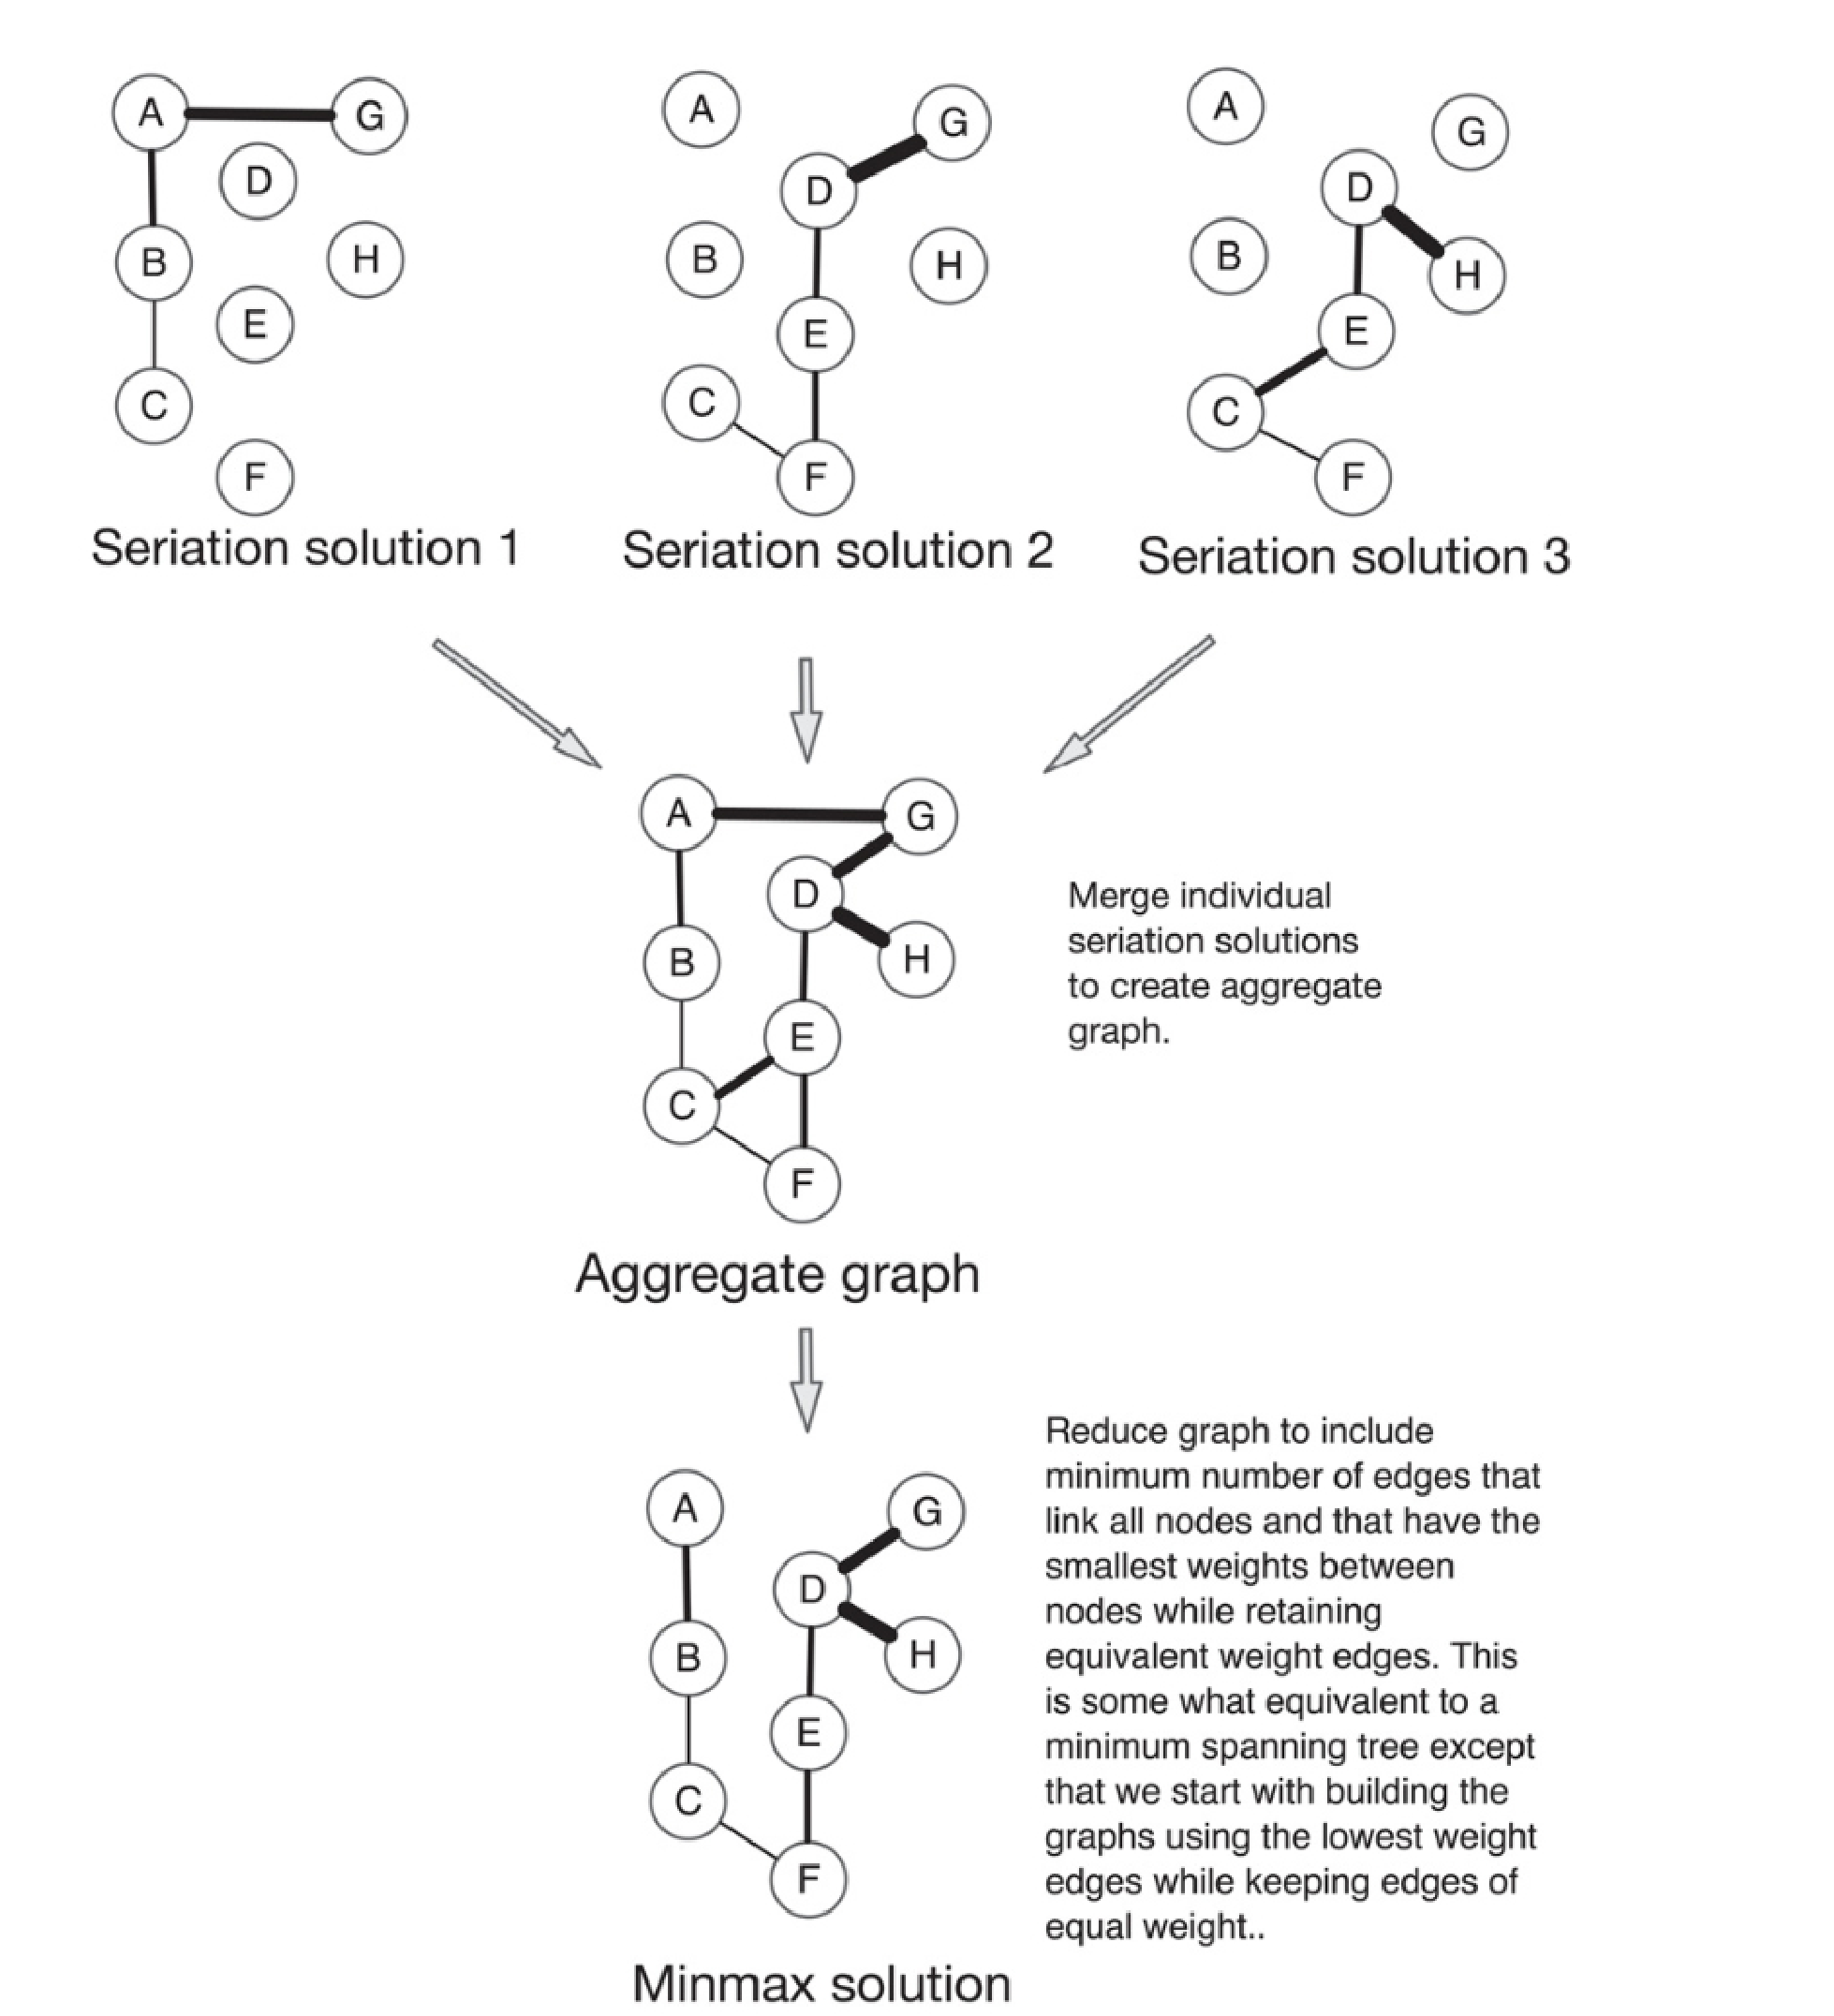
\includegraphics[scale=0.4]{graphics/conclusion/lipo2015-figure6-minmax.pdf}
  \caption{Seriation graph creation steps.  In this example, we begin with the graph representation of three valid seriation solution fragments (1-3) for a set of 9 assemblages (A-I).  In the figure, the thickness of the edges reflects the summed difference in frequencies between each pair of assemblages.  Each solution represents a valid and unique seriation.  To combine these three possible solutions into one overall solution, we first take the union of the partial graphs to create a single aggregate solution that is composed of all vertices and edges from the individual subsolutions.  Using the aggregated graph or ``sumgraph'', we then reduce to a final seriation solution by including the fewest edges that can be made between all vertices and starting with the edges with the smallest weight (the sum of frequency differences).  Edges are added sequentially ranked by total frequency difference until the vertices form a single connected three.  Edges with equivalent total weight are retained.  Reprinted from Figure 6, \citep{Lipo2015} under the terms of the Creative Commons Attribution License \url{https://creativecommons.org/licenses/by/4.0/}.}
  \label{conc:fig:minmax-seriation}
\end{figure}

Second, it is possible to study other representations of seriation data as well which might contain more structure.  Our IDSS seriation algorithm \citep{Lipo2015} by default produces solutions which represent the ``minmax'' solution:  the largest set of assemblages that can form a valid solution, linked by edges which represent the smallest differences between class frequencies among adjacent vertices (Figure \ref{conc:fig:minmax-seriation}).  This ``minmax'' solution graph, whether constructed using unimodality as the ordering criterion or simple distance minimization (as described in Chapter \ref{chap:multipleseriation-paper}), represents a kind of minimal spanning tree which accounts for both spatial and temporal effects on ordering assemblage frequencies.  

That minimum spanning tree is constructed by \emph{pruning} edges from an intermediate representation which is the union of all valid subsolutions (Lipo and I dubbed this the ``sumgraph'' or ``aggregrate'' graph representation).  If the criterion being used is unimodality, the sumgraph will represent only those links where unimodal solutions could be found, and will be denser than a tree but sometimes sparser than the complete graph over N vertices.  The sumgraph records more similarity information than a ``minmax'' solution tree, and can have loops, cliques, and richer overall structure.  Because the graph structures are not strict trees, and can have richer connectivity patterns (which can vary in different areas of the solution), the Laplacian spectra should exhibit more variation.  This creates a large space of variation within which we might distinguish between hypotheses in assessing equifinality, and potentially clearer ability to fit empirical data to different models.  I have done some work repeating the experiments of Chapter \ref{chap:computational-metapopulation} with sumgraphs rather than minmax seriation trees, and the results seem promising but there is a great deal that can be done to extend this line of research.  

\subsection{Classification and Modeling Design Space}\label{conc:sec:future-design-space}

We always measure cultural variation, and map its spread through space and history through time, by examining the prevalence of archaeological classes of types \citep{Dunnell1971}.  These classes are always analytical constructions, even if in practice archaeologists frequently employ standard classifications in a given region whose origins are a mixture of analysis and common sense.  Since those classes are constructions, it is clear that ``Baytown Plain'' or ``Elko corner-notched'' are not really units of transmission, in the sense that the attributes denoted by those types were always learned or copied together.  And yet, in much of the published literature on cultural transmission modeling in archaeology, we end up treating types as if they were units of transmission.  This false equivalence causes us to ignore the actual levels at which cultural information is being transmitted---sometimes at the level of whole artifacts, sometimes at the level of individual attributes, and at levels in between given that individuals often learn \emph{techniques} for construction and the attributes we observe are the byproducts of employing those techniques.  

\begin{figure}[ht!]
  \centering
  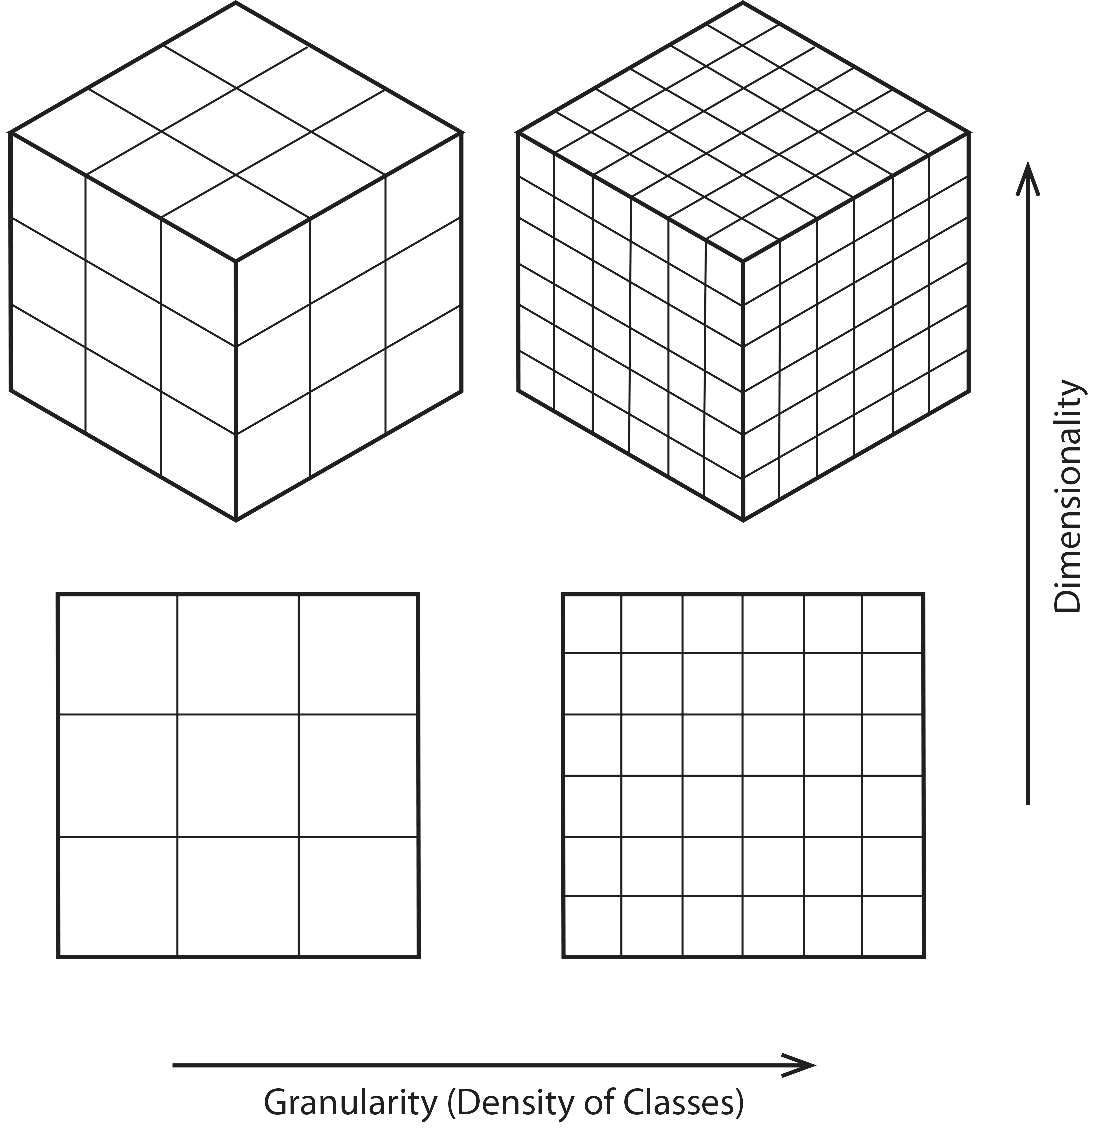
\includegraphics[scale=0.5]{graphics/conclusion/classification-granularity-dimensionality.pdf}
  \caption{Factors which govern classification ``level''.}
  \label{conc:fig:classification-granularity}
\end{figure}

Instead, we should  explicitly model the effects of classification and its ``level'' (fineness or coarseness) on our transmission models, in the same fashion that in Chapters \ref{chap:ctmixtures-paper} and \ref{chap:computational-metapopulation} I explicitly modeled temporal aggregation in the transmission model itself.  We can do this by  modeling the artifact design space as a paradigmatic classification \citep{Dunnell1971,OBrien2015}.  Given a well constructed paradigmatic classification, we can vary the ``fineness'' with which we tabulate cultural variation by changing the ``level'' of the classification:  adding or removing dimensions, or changing the granularity with which we slice a dimension of variation into attributes or modes (see Figure \ref{conc:fig:classification-granularity}).  In our early work \citep{Lipo1997}, we changed the level of the Phillips et al. ceramic classification for the Lower Mississippi River Valley by lumping their types into larger aggregates, and performed seriations with the original and two levels of lumped classifications.  When the resulting seriation solutions were mapped, the effect of varying the level of the classification is to create clusters of assemblages at different levels of spatial detail \citep[Fig. 17]{Lipo1997}.  Thus, changing the level of classification has the effect of revealing different levels of detail about the evolutionary history of variants, giving us a limited ability to ``zoom in'' or out to see pattern at different spatiotemporal scales.

Adding data collection treatments like assemblage sampling, time averaging, and variable classification level to a simple cultural transmission model adds a great deal of overhead and complexity.  In the research described in Chapter \ref{chap:computational-metapopulation} I elected not to include classification level in the simulation models because the computational requirements of the model were already very challenging, and slowing things down even further would have led to even smaller numbers of replicates.  But that is a software engineering problem, not a scientific one.  I have examined how to add variable classificatory level to our simulation models, and extending the work in Chapter \ref{chap:computational-metapopulation} to include it is a necessary next step.\footnote{A framework for tracking a simulation with a variable-level classification exists in the open-source repository \url{https://github.com/mmadsen/ctpy}, with a fuller Java-based implementation in \url{https://github.com/mmadsen/TransmissionFramework} that can be ported to Python for integration into the SimuPOP-based simulations described in this dissertation.}.


\subsection{Next Steps on Modeling Structured Information}\label{conc:sec:structured-next-steps}

The vast bulk of research on cultural transmission modeling in archaeology has been concerned with \begin{dissparalist}
\item what the frequency distribution of classes implies about selection or cognitive biases
\item what class frequencies can tell us about interaction in space and time.
\end{dissparalist}  These problems, at least as originally framed, required only very ``thin'' descriptions of cultural variants.  In other words, cultural variants in most of our models are simply markers, that possess counts and frequencies.  This is to be expected, given the nature of the questions being asked.  But answering questions about how technologies evolve through selection, social learning, and individual innovation require somewhat ``thicker'' descriptions in our models.  As Gilbert Tostevin \citeyearpar{tostevin2019content} has argued, the \emph{content} of cultural traits matter when constructing transmission models.

Modeling the content of cultural traits in terms of cultural transmission means recognizing that traits bear a variety of relationships to each other \citep{mesoudi2008learning}.  Flake types in lithic assemblages relate to each other in terms of reduction sequences; the unpainted color of ceramic vessels is related to firing temperature and firing atmosphere, and so on.  Attributes of technologies are related in terms of the steps needed to create a finished product, the prerequisite knowledge and skill the artisan needs to perform a given technological transformation, and the locations, resources and other ``scaffolding'' needed to learn and execute it \citep{wimsatt2007reproducing,wimsatt2019articulating}.  Thicker descriptions are important in order to employ cultural transmission models to answer questions about the substantive history of technologies, although they are vital in this role.   

In Chapter \ref{chap:semanticaxelrod-paper} I attempted to model one type of dependency between traits:  attributes that represent knowledge which is prerequisite to learning, and thus being able to execute, other attributes.  I employed the tools of algebraic graph theory to examine the degree to which the pool of variation in observed assemblages fills the abstract ``design space''.  I believe the framework has merit, but there are more relationships and dependencies that can and should be modeled.  \citet{premo2016cultural} describe how different classes might be observed, learned, and imitated in different ways in different locations, leading to their idea of the ``taskscape''.  Traits or classes which are only observable in certain restricted contexts may exhibit more variability at a regional scale than those which are observable easily in many contexts, for example.  

A good next step would be to examine whether the analysis from Chapter \ref{chap:semanticaxelrod-paper} could be done in the context of a model of lithic reduction sequences, and refine the symmetry analysis methods used there to examine how the ``design space'' for reduction sequence options fills in over time, and varies regionally.  This kind of analysis would require, and lead to, deeper partnerships between specialists in different classes of prehistoric technologies, and specialists in evolutionary modeling.  

But a word of caution is in order.  As we develop more realistic models for dependencies between traits, we will need to be on our guard not to feel the ``pull of the synchronic''.  There is merit in looking at how social learning interacts with the structure of a technology, but we should not fool ourselves into thinking that we are going to understand how flintknappers in the middle Paleolithic learned their craft, any more than we're going to learn how much Neolithic European potters were conformists or novelty-seekers.  Our goal in thicker models for the transmission of technology should still be to understand change and build diachronic measures for change and innovation.  A focus on classification, modeling of the design space and dependency relationships, and then building hypotheses about how design space is explored over time, should help keep our modeling efforts firmly at archaeological scales. 

\section{Final Thoughts}\label{conc:sec:final-thoughts}

Cultural transmission, broadly understood, is the backbone of an evolutionary archaeology; through the principle of heritable continuity it provides the central organizing framework for the construction of evolutionary chronicles; and provides the mechanism through which other evolutionary processes act as part of our evolutionary explanations.  Our exploration of cultural transmission theory and models in archaeology is, perhaps, out of its infancy, but principally because we have begun to explore its failures and limitations.  

\begin{figure}[ht!]
  \centering
  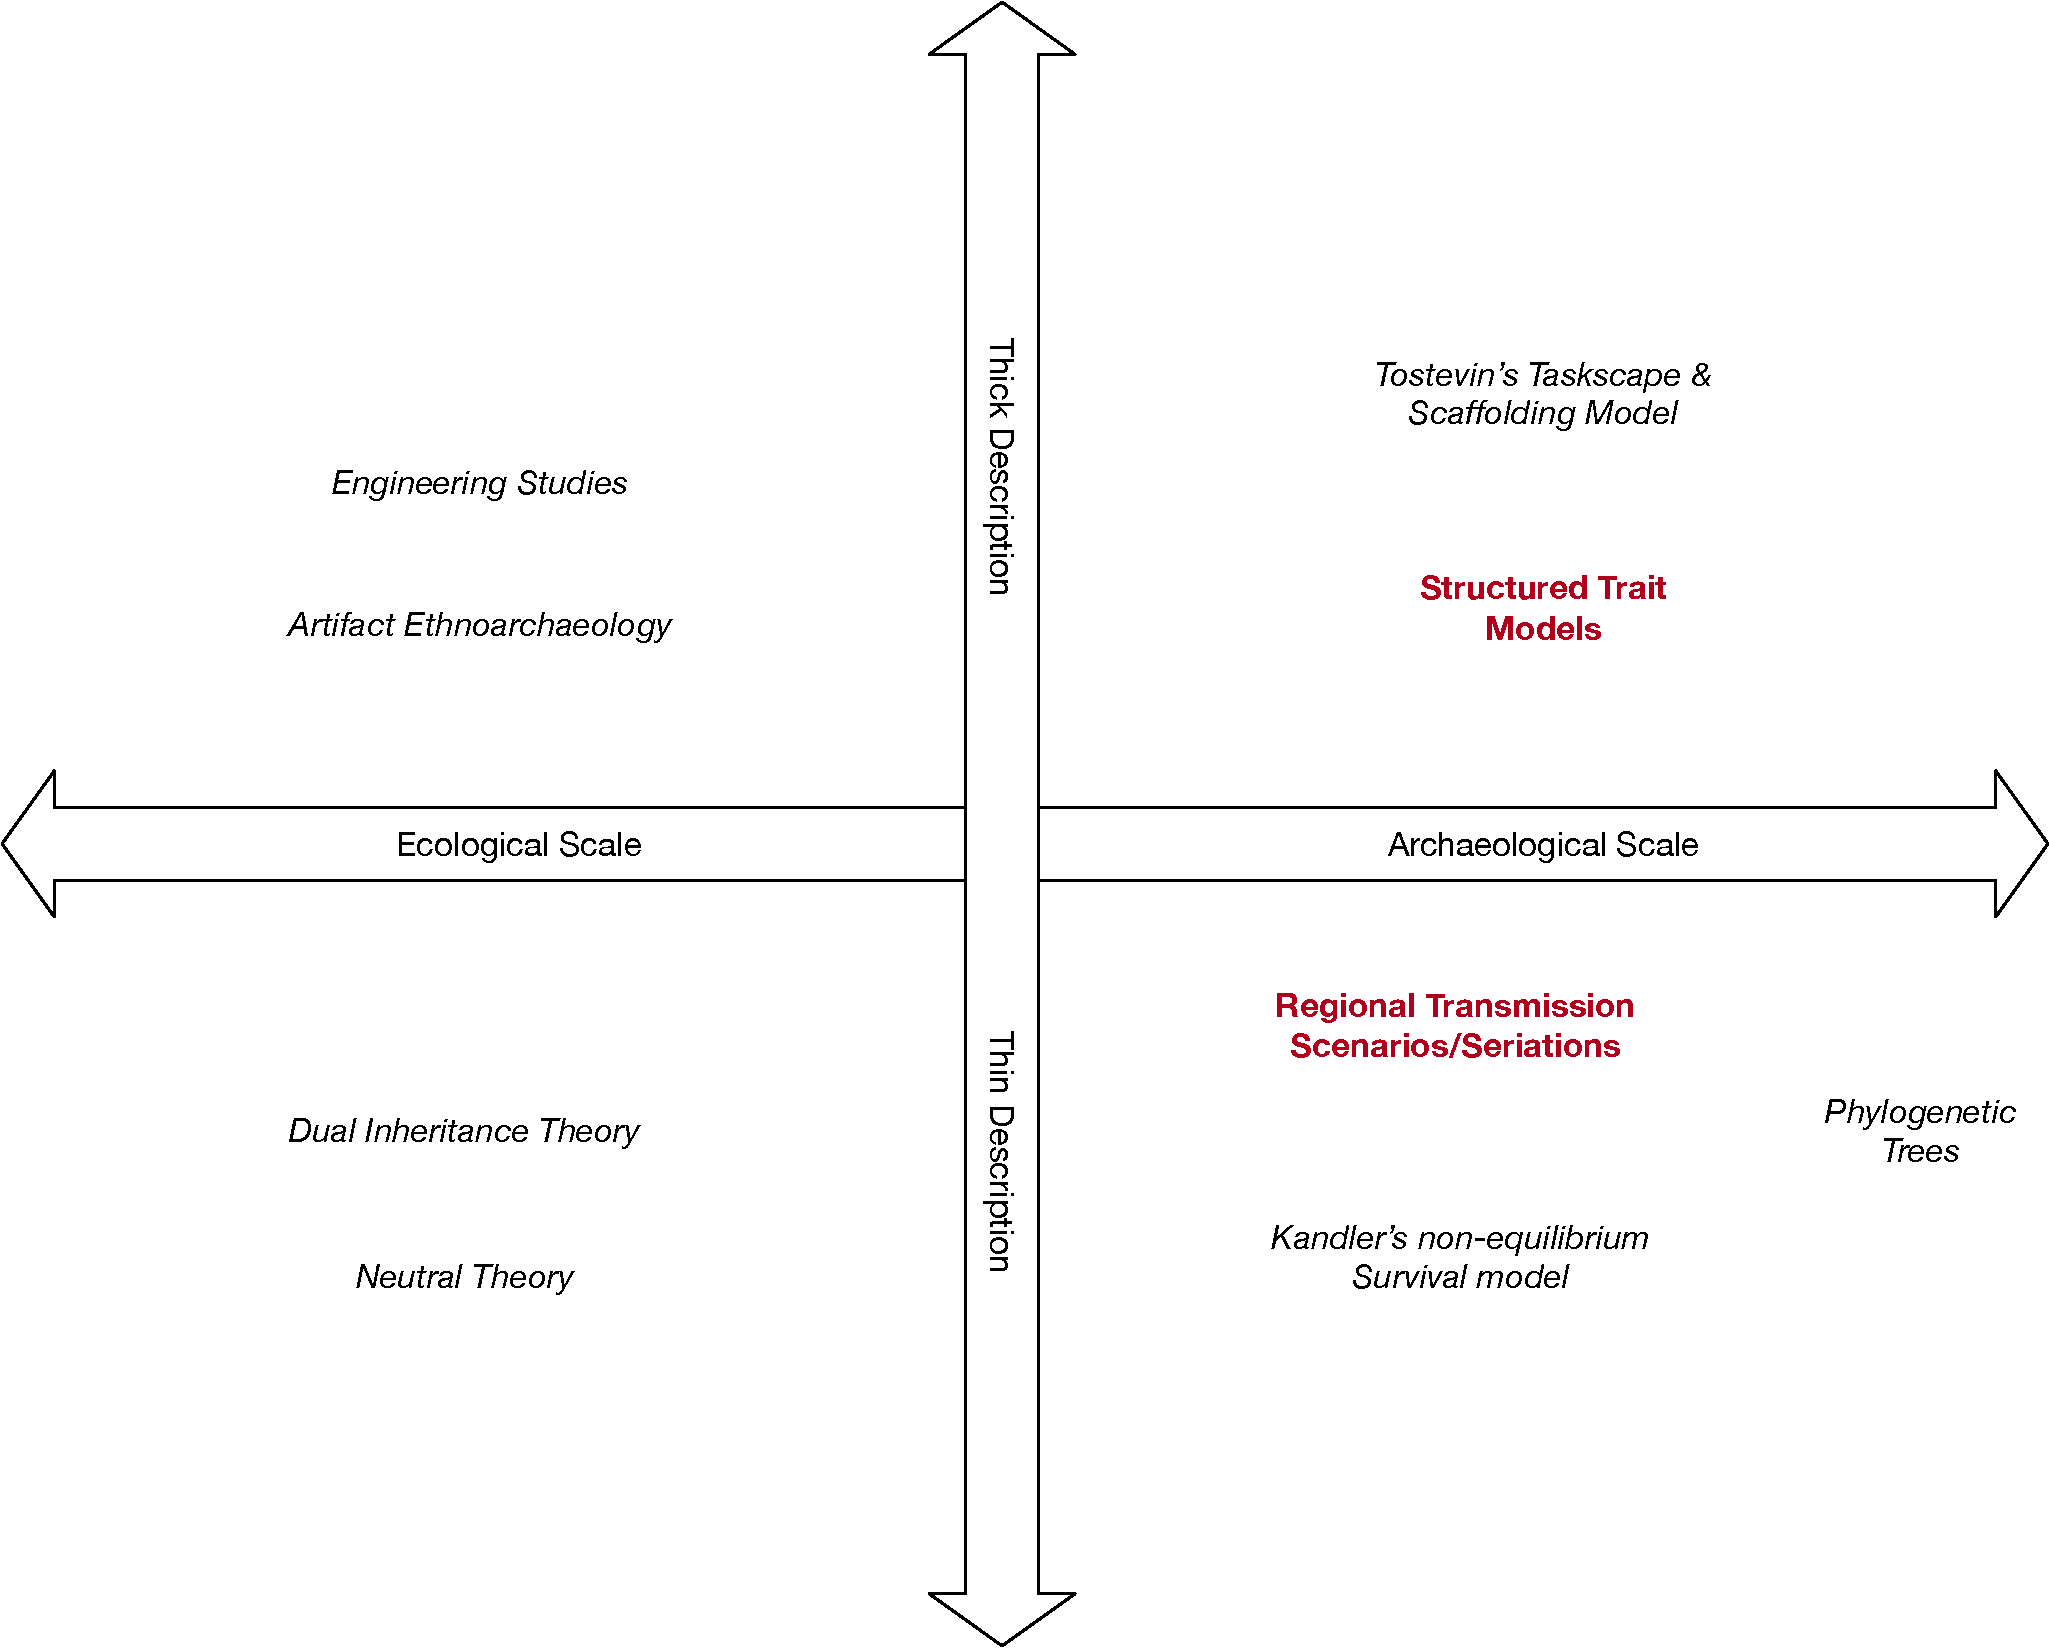
\includegraphics[scale=0.5]{graphics/conclusion/quadrant-diagram.pdf}
  \caption{Conceptual relationship between the models and research discussed in this dissertation and cultural transmission studies within archaeology.  The horizontal axis describes the time scale over which a body of theory of models are operative, from synchronic, ``ecological time'' models on the left, through diachronic, time averaged, ``archaeological scale'' models on the right.  The vertical axis describes how ``thin'' or ``thick'' a model or theory is; does it treat cultural variants as abstract markers, or does it incorporate the ``semantics'' of how traits fit together:  dependencies, engineering relationships, and prerequisites?  The author's research in this dissertation is highlighted in red, to situate the work among other approaches.}
  \label{conc:fig:quadrant-diagram}
\end{figure}

Although I conclude in this work that evolutionary archaeologists should give up on the microevolutionary program given its conceptual and empirical weaknesses, the enterprise of building mathematical models of social learning and constructing statistical methods for fitting them to data is absolutely critical.  Those data will simply not be archaeological, in most cases.  But we still need to understand how cultural transmission ``works'' as a system of heritability.  Conclusions from theory building and studies at ecological scales can inform the theory building and studies we do at archaeological scales without being directly ``renormalizable'' between scales, or direct statistical fitting exercises.  The relationship is instead much the same relationship that population genetics and evolutionary ecology have with paleobiology.  

In Figure \ref{conc:fig:quadrant-diagram}, I attempt to depict the relationship between the various research programs and models discussed in this dissertation.  The horizontal axis principally reflects time scale, from ecological scale studies of living populations, to archaeological scales which cover broad spans of space and time.  The vertical axis reflects the degree to which cultural transmission models are ``thin'' and study just the statistical distribution of outcomes, or are ``thicker'' and model the actual content and relationships of cultural traits.  The ``mesoscale'' research and  models discussed in this dissertation are shown in red.  The areas of theory and modeling given on the left side function as the synchronic science that the right hand side can use to build diachronic chronicles and evolutionary explanations. 

On the right hand side, we need both thin and thick efforts, for different purposes.  The purpose of ``thin'' models at archaeological scales is to map the \emph{flow} of cultural variation through space and time.  Thin models give us the evolutionary chronicle of what happened when, where the innovations came from, to where did they spread, where they were adopted, where they were abandoned after they proved less than useful, and so on.  Thick models take the engineering and functional information we derive from essentialist sciences like physics, chemisty, and various engineering disciplines, as well as rigorous ethnographic observations, to help us explain \emph{how} technologies evolved, by allowing us to see our artifact classes (and their shifting frequencies) in the overall context of the technologies of which they are the phenotypic ``hard parts''.  

On the right side of the diagram, I included several other bodies of research that are important for elaborating a truly archaeological scale cultural transmission theory.  I have described the importance of Kandler's \citeyearpar{Kandler2013} work on non-equilibrium, diachronic models elsewhere in this work, as well as Tostevin's \citeyearpar{tostevin2012seeing,tostevin2019content} work developing rich models for the social learning of lithic technology.  Both pieces of work serve as exemplars of approaches we need to follow.  

Phlyogenetic methods, and the macroevolutionary approach based upon them, have received less attention in this dissertation, but it is appropriate to understand their relationship to the ``mesoscopic'' work described here on seriation.  I do not see seriation and cladistics as competitors or alternatives.  They are, instead, ends of a continuum of methods for documenting the evolutionary chronicle.  This continuum operates by varying \emph{classificatory level} principally, and by using categorical versus ratio scale variables.  Although there has been some work on polymorphic phylogeny, employing frequencies of traits to understand finer-scale phylogenetic relationships \citep{Wiens1999}, the vast bulk of phylogenetic analysis employs the presence or absence of classes or traits (and their directionality of change, in cladistics) to determine relationships between taxa or samples.  Seriation, both as classically employed and as rebuilt by Lipo and myself as an evolutionary method, can employ both presence/absence and frequencies, but most often employ class frequencies.  

Given these similarities and differences, it is typical that seriation is most appropriate when most assemblages or samples share the same group of classes (even if not all assemblages possess all classes), and where the differences arise in their frequency.  Such situations are ``zoomed in'' often to relatively small intervals of time and small regions.  This is the ``mesoscale'' as discussed in this dissertation.  Phylogenetic methods are most appropriate when most assemblages or samples do not share the same group of classes, and we seek to understand evolutionary history simply through the pattern of their innovation and adoption.  That is typically at larger spatial and longer time scales than questions we employ seriation to answer.  The methods---and future derivatives of each, since there is much room for innovation here---are like selecting different lenses for a camera, rather than using different tools altogether.  There will be much fruitful cross-pollination between the methods as well if we stop seeing them as alternatives or different methods and begin seeing them as a continuum of ways to create testable and secure evolutionary chronicles.

In the final analysis, evolutionary archaeology .....
